\section{Benchmarking PCPOP}
\label{sec:benchmark}
We report the performance of PCPOP on examples considered before. We use the size of the principal moment matrix, number of scalar variables and cpu time as measure of performance on a problem at specific level of relaxation.

We start with the example \ref{ex:pcpop_hardy} as it can be generalized to any number of parties to show genuine multipartite entanglement.

\begin{table}[H]
	\centering
	\caption{Benchmark summary for PCPOP relaxations. SDP size refers to the principal moment matrix dimension; CPU time measured in milliseconds.}
	\label{tab:pcpop-bench}
	\begin{tabular}{@{}ccrrr@{}}
		\# of parties & level & SDP size & \# scalar vars& CPU time (ms) \\
		\midrule
		% Fill rows below with your data
		% parties  order  size  vars  time(ms)
		2 & 2 & 13 & 31 & 10.658 \\
		2 & 3 & 25 & 61 & 31.803 \\
		2 & 4 & 41 & 101 & 119.239 \\
		3 & 2 & 25 & 93 &  46\\
        3 & 3 & 63 & 250 & 571.962 \\
        3 & 4 & 129 & 529 & 13165 \\
        4 & 2 & 41 & 229 & 226.255 \\
        4 & 3 & 129 & 833 & 14491 \\
        4 & 4 & 321 & 2241 & 323277 \\ 
		\bottomrule
	\end{tabular}
\end{table}
Now, we compare the performance of PCPOP with Ncpol2sdpa on the examples $\ref{ex:3comms},\ref{ex:4comms},\ref{ex:5comms}$. We compare the size of the principal moment matrix and the number of scalar variables for both packages at the same relaxation order.
\begin{table}[H]
	\centering
	\caption{Comparison of PCPOP and Ncpol2sdpa by relaxation order. SDP size refers to the principal moment matrix dimension.}
	\label{tab:compare-pcpop-ncpol}
	\begin{tabular}{@{}cccrrr@{}}
		\toprule
		Example & level & Gr\"obner size & Package & SDP size & \# scalar vars \\
		\midrule
		\multirow{2}{*}{\ref{ex:3comms}} & \multirow{2}{*}{2} & \multirow{2}{*}{6} & PCPOP      & 9 & 23 \\
		                           &                    &                      & Ncpol2sdpa & 9 & 25 \\
		\addlinespace
		\multirow{2}{*}{\ref{ex:3comms}} & \multirow{2}{*}{3} & \multirow{2}{*}{8} & PCPOP      & 17 & 58 \\
		                           &                    &                      & Ncpol2sdpa & 18 & 73 \\
		\addlinespace
        \multirow{2}{*}{\ref{ex:3comms}} & \multirow{2}{*}{4} & \multirow{2}{*}{10} & PCPOP      & 30 & 142 \\
		                           &                    &                      & Ncpol2sdpa & 35 & 223 \\
		\addlinespace

		\multirow{2}{*}{\ref{ex:4comms}} & \multirow{2}{*}{2} & \multirow{2}{*}{10} & PCPOP      & 15 & 60 \\
		                           &                    &                      & Ncpol2sdpa & 15 & 64 \\
		\addlinespace
		\multirow{2}{*}{\ref{ex:4comms}} & \multirow{2}{*}{3} & \multirow{2}{*}{14} & PCPOP      & 37 & 219 \\
		                           &                    &                      & Ncpol2sdpa & 40 & 284 \\
		\addlinespace
        \multirow{2}{*}{\ref{ex:4comms}} & \multirow{2}{*}{4} & \multirow{2}{*}{18} & PCPOP      & 82 & 723 \\
		                           &                    &                      & Ncpol2sdpa & 96 & 1339 \\
		\addlinespace
		\multirow{2}{*}{\ref{ex:5comms}} & \multirow{2}{*}{2} & \multirow{2}{*}{13} & PCPOP      & 24 & 176 \\
		                           &                    &                      & Ncpol2sdpa & 24 & 184 \\
		\addlinespace
		\multirow{2}{*}{\ref{ex:5comms}} & \multirow{2}{*}{3} & \multirow{2}{*}{19} & PCPOP      & 85 & 1686 \\
		                           &                    &                      & Ncpol2sdpa & 89 & 1934 \\
		\addlinespace
		\multirow{2}{*}{\ref{ex:5comms}} & \multirow{2}{*}{4} & \multirow{2}{*}{25} & PCPOP      & 287 & 17226 \\
		                           &                    &                      & Ncpol2sdpa & 315 & 22126 \\
		\bottomrule
	\end{tabular}
\end{table}
On top of improvements in the size of the principal moment matrix and number of scalar variables, PCPOP also provides tighter bounds as compared to Ncpol2sdpa. This is obvious as PCPOP imposes more constraints on th emoment matrix.
\subsection{PCPOP vs OSCAR and QuantumNPA}
OSCAR~\cite{OSCAR} is an excellent computer algebra system implemented in Julia. It implements Grobner basis computation and reductions for various algebras. For specific examples \ref{ex:partial_comms}, we compare the performance of PCPOP with OSCAR and PCPOP with QuantumNPA in finding normal forms. OSCAR first needs to compute the Grobner basis and then use it to reduce monomials/polynomials to their normal forms. 
\begin{example}
	\label{ex:partial_comms}
	Here we will consider set of variables $V = \{x_1, x_2, \ldots, x_{3*n}\}$ where the variables $V$ can be partitioned into 3 groups of n variables each say $A=\{x_1,x_2 \ldots x_n\}$, $B=\{x_{n+1},x_{n+2} \ldots x_{2*n}\}$ and $C=\{x_{2*n+1},x_{2*n+2} \ldots x_{3*n}\}$. Every variable in group A commutes with every variable in group B  and every variable in group B commutes with every variable in group C. However, no variable in group A commutes with any variable in group C.
\end{example}
 Note that for the example~\ref{ex:partial_comms}, OSCAR needs to find Grobner basis up to degree $d$ to reduce monomials of degree $d$. PCPOP on the other hand builds the partially commutative monoid structure once and can reduce monomials of any degree. This makes PCPOP and also QuantumNPA better than OSCAR atleast for equalities including partial commutations and binomial constraints (projectors, unitary \dots). We provide time taken by OSCAR to find Grobner basis and time taken by PCPOP to build the partially commutative monoid structure. We also provide time taken by OSCAR, PCPOP and QuantumNPA to reduce random monomials of increasing degree to their normal forms.
In figure~\ref{fig:partial_comms_reduction}, we benchmark the time taken to compute normal forms of $m*m$ where m is a random monomial of degree $d$ for increasing values of $d$. 

\begin{figure*}[t!]
    \centering
    \begin{subfigure}[t]{0.5\textwidth}
        \centering
		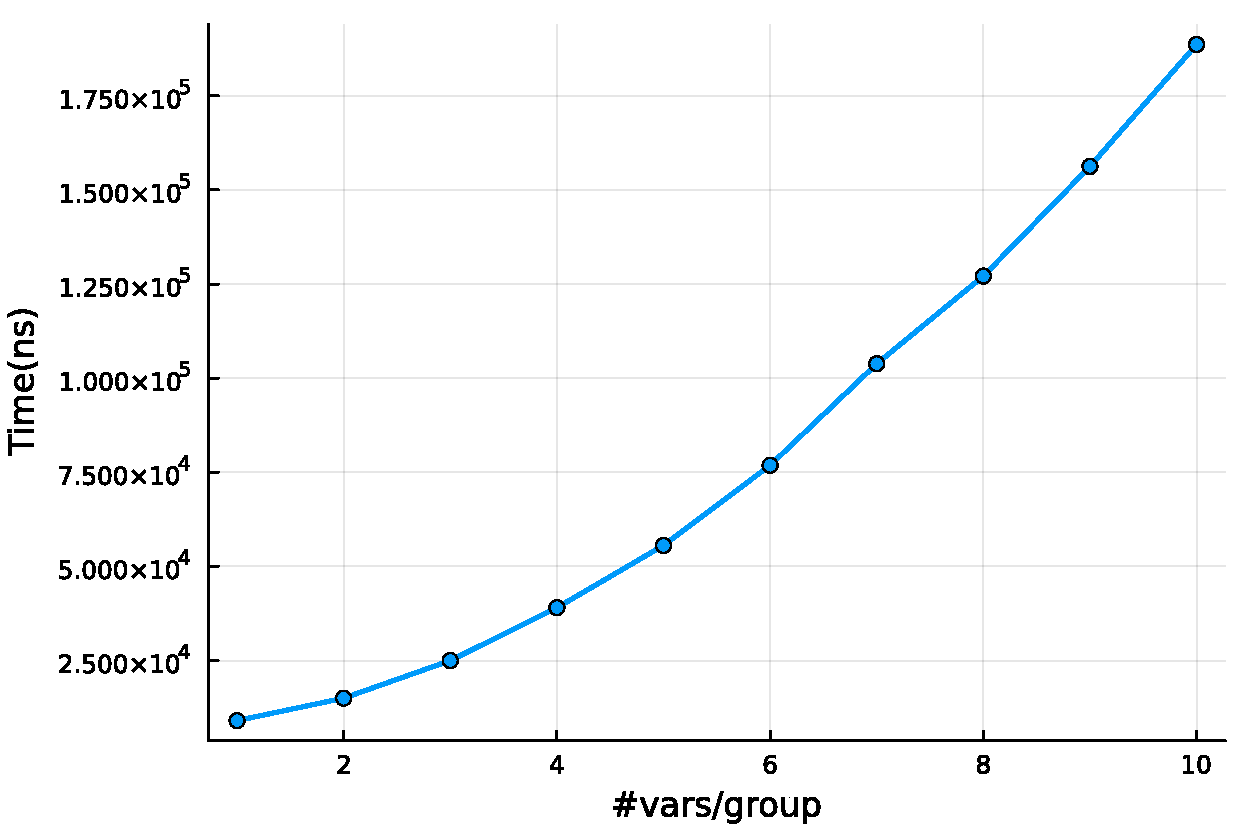
\includegraphics[width=\textwidth]{./../Benchmark/plots/benchmark1/startup/M.pdf}
        \caption{Time PCPOP takes to build the partially comm. monoid}
    \end{subfigure}%
    ~ 
    \begin{subfigure}[t]{0.5\textwidth}
        \centering
		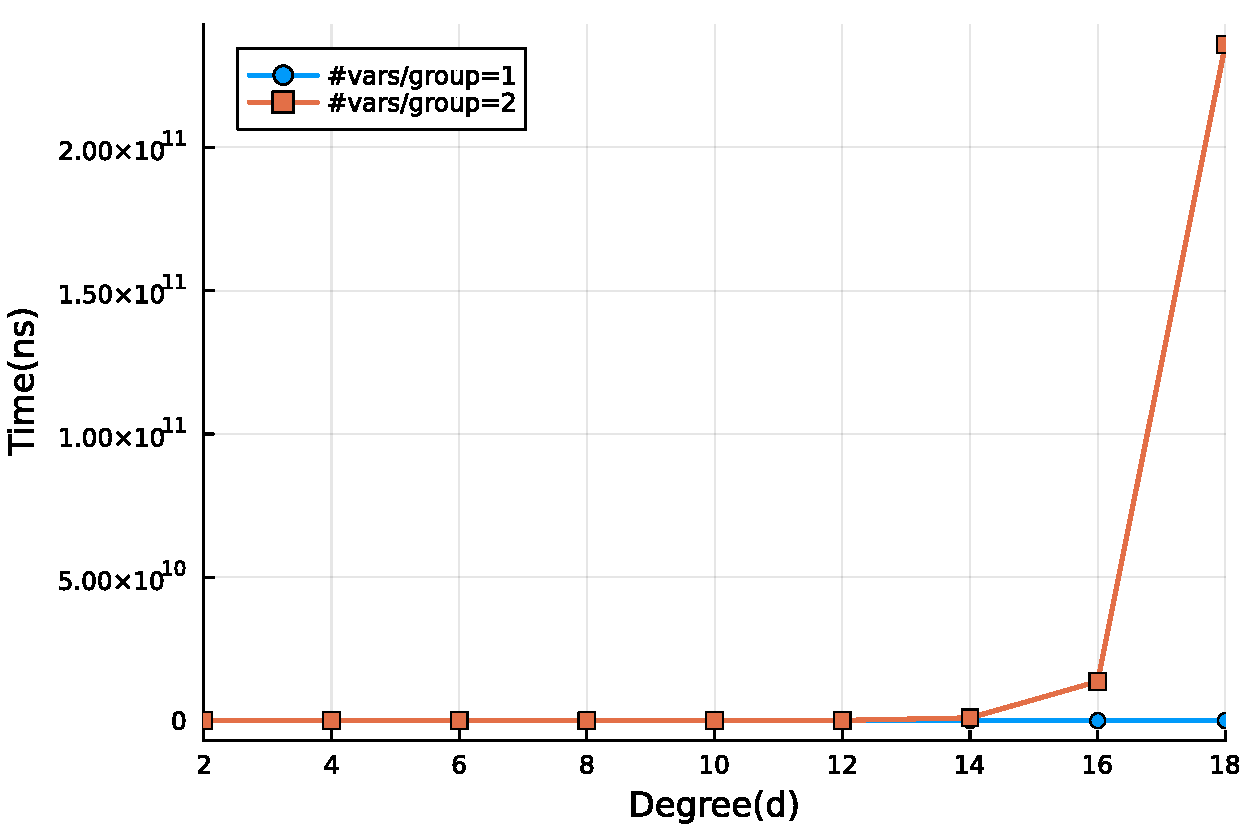
\includegraphics[width=\textwidth]{./../Benchmark/plots/benchmark1/startup/gvars1vs2.pdf}
		\caption{Time OSCAR takes to compute the GB}
    \end{subfigure}
	\caption{}
\end{figure*}


\begin{figure*}[t!]
    \centering
    \begin{subfigure}[t]{0.5\textwidth}
        \centering
		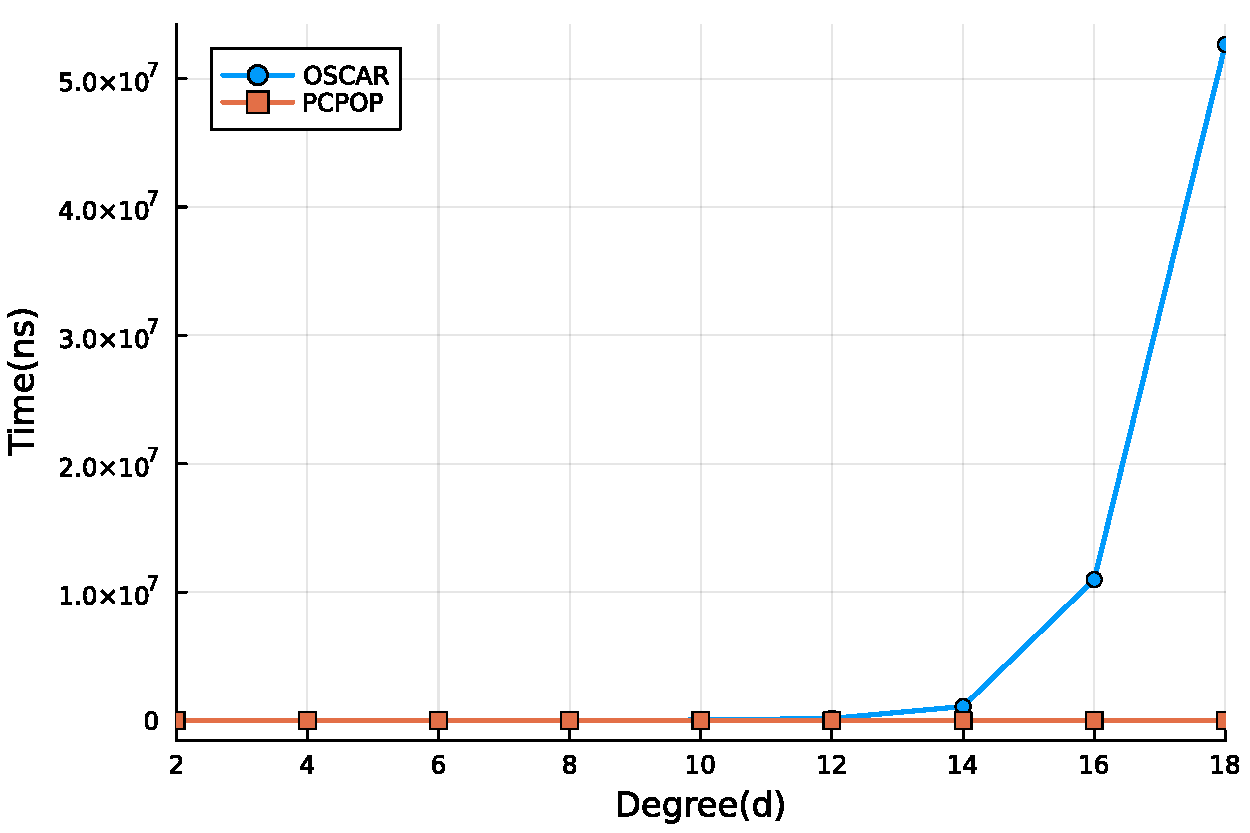
\includegraphics[width=\textwidth]{./../Benchmark/plots/benchmark1/normal_form/OSCARvsPCPOP_vars=2.pdf}
		\caption{Example 10: Comparision of PCPOP vs OSCAR.}
    \end{subfigure}%
    ~ 
    \begin{subfigure}[t]{0.5\textwidth}
        \centering
		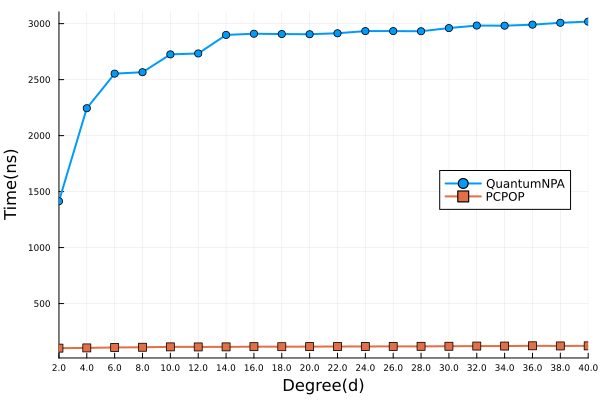
\includegraphics[width=\textwidth]{./../Benchmark/plots/benchmark1/normal_form/QuantumNPAvsPCPOP_vars=2.png}
		\caption{Example 10: Comparision of PCPOP vs QuantumNPA.}
    \end{subfigure}
	\caption{For both plots the number of variables in each group i.e n is 2.}
		\label{fig:partial_comms_reduction}
\end{figure*}


 \begin{example}
	\label{ex:partial_comms_with_projectors}
	In this example we have same variables and commutations as before but in addition all the variables $x_i$ are projectors i.e $x_i^2 = x_i$.
 \end{example}
As before, we compare the performance of PCPOP with OSCAR and PCPOP with QuantumNPA in finding normnal forms for example~\ref{ex:partial_comms_with_projectors} in figure~\ref{fig:partial_comms_projs_reduction}.

\begin{figure*}[t!]
    \centering
    \begin{subfigure}[t]{0.5\textwidth}
        \centering
		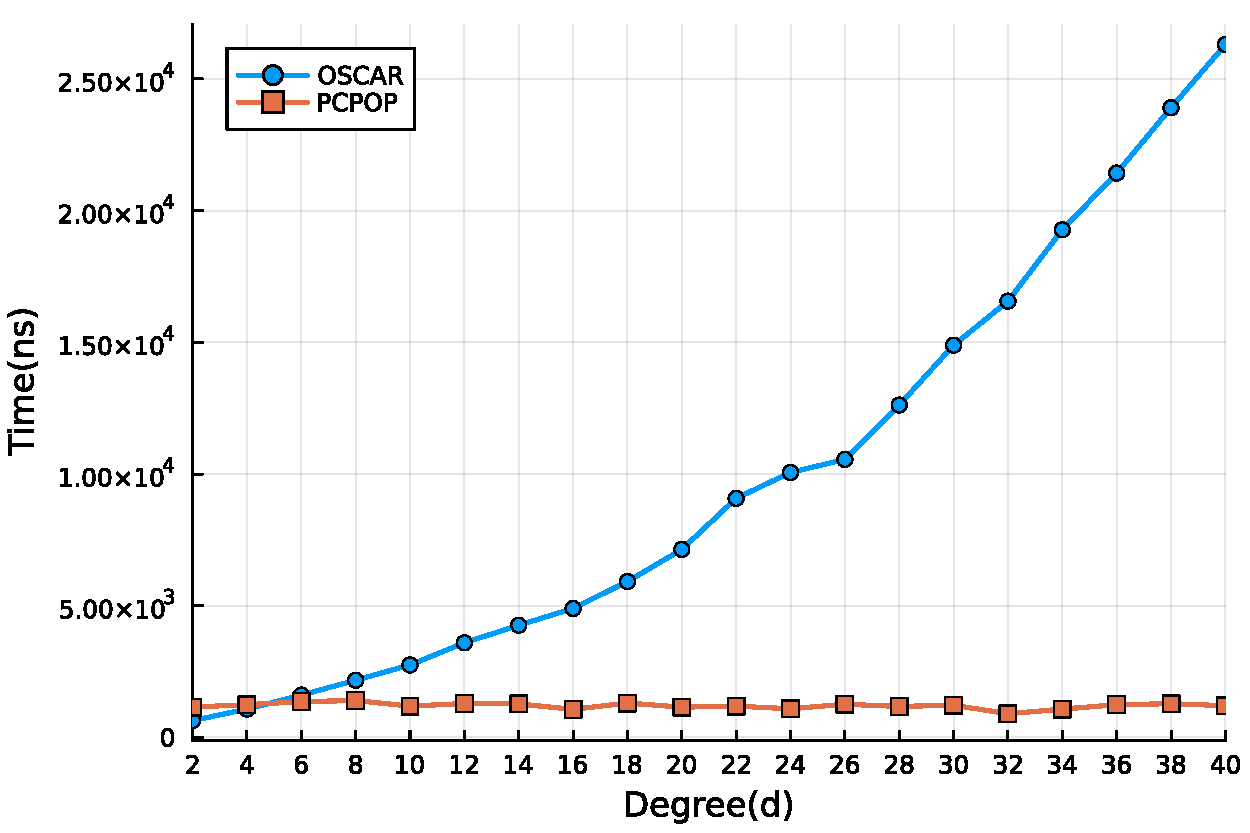
\includegraphics[width=\textwidth]{./../Benchmark/plots/benchmark2/normal_form/OSCARvsPCPOP_vars=2.pdf}
		\caption{Example 11: Comparision of PCPOP vs OSCAR.}
    \end{subfigure}%
    ~ 
    \begin{subfigure}[t]{0.5\textwidth}
        \centering
		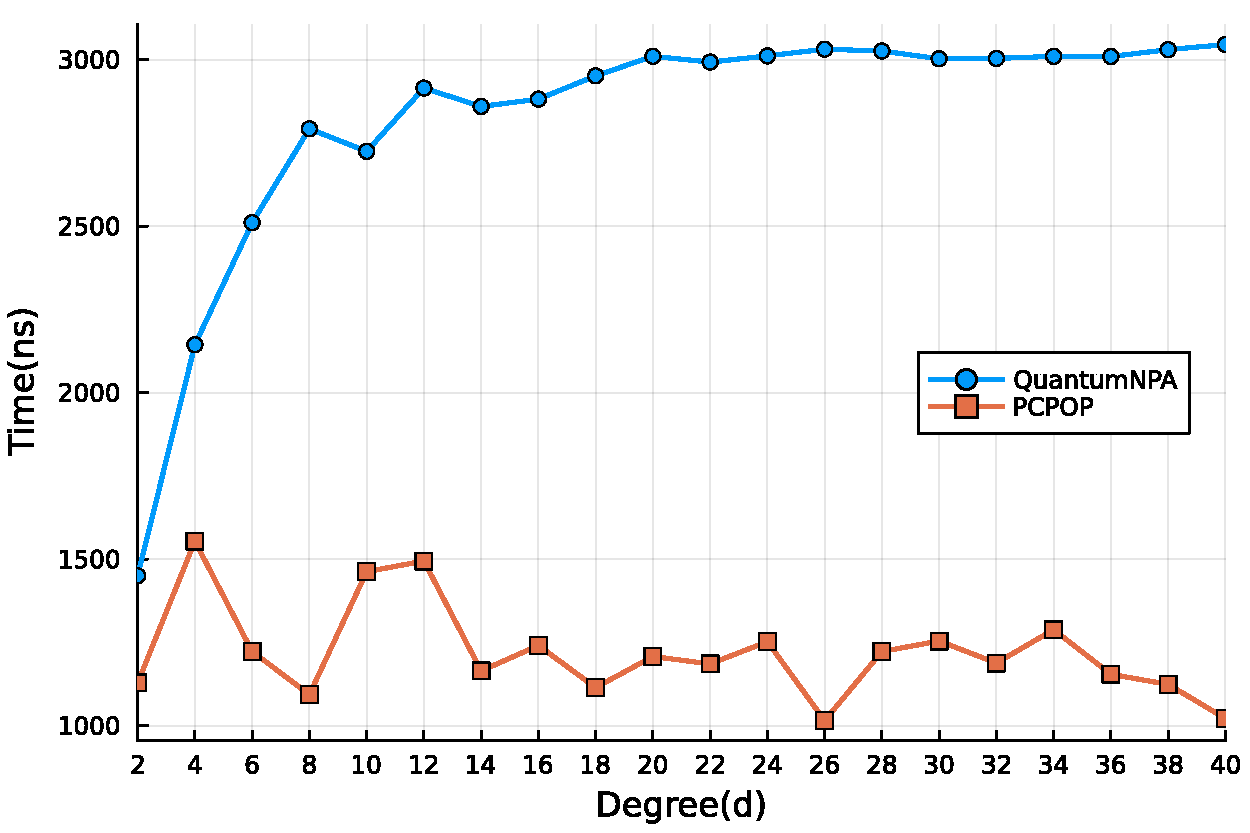
\includegraphics[width=\textwidth]{./../Benchmark/plots/benchmark2/normal_form/QuantumNPAvsPCPOP_vars=2.pdf}
		\caption{Example 11: Comparision of PCPOP vs QuantumNPA. }
    \end{subfigure}
	\caption{For both plots the number of variables in each group is 2.}
		\label{fig:partial_comms_projs_reduction}
\end{figure*}

